\section{Autoparametric Oscillator Solutions}
% \label{S:engr}

% We now look at various quantities of engineering interest; to do so, we start with the fact that due to the symplectic nature of the transformation
% \[
% \iiiint f(x_1,x_2,x_3,x_4) dx_1 dx_2 dx_3 dx_4 = \int d\psi\int dI \int dh \oint_{E(h,I)} \frac{f(u,I,\psi)}{\|\nabla H \|} ds
% \label{E:quarticint}
% \]
% where
% \[
% E(h,I) \equiv \left\{ u \in \Real^2 : H(u, I)=h \text{ and } I = \text{constant} \right\},
% \]
% and the arc length $s$ of the curve $E(h)$ is the new variable of integration. In adition if $f(u,I,\psi) = f(H(u,I),I)$, then the integral on the right hand side yields
% \[
% \int f(h,I) dh dI\oint_{E(h,I)} \frac{ ds}{\|\nabla H \|} = \int f(h,I) \period_H(h,I) dh \, dI
% \]
% Hence, an appropriate inner product in the local coordinate $z=(h,I)$ is given by
% \[
% \left\langle f(z), g(z) \right\rangle_{H,I} \equiv
% \int_{H=h} \int_{I=\text{constant}} f(z) \, g(z) \; \period (z) \;
% dh\, dI
% \]

% \subsection{Derivation of the Fokker-Planck Equation}

% Now we derive the Fokker-Planck equation (FPE) for the density of $\{\yen_{t \wedge \check{\mathfrak{e}}}; t \geqslant 0\}$ or equivalently $\{(\check h_{t\wedge \check{\mathfrak{e}}}, \check{I}_{t\wedge \check{\mathfrak{e}}});$ $t \ge 0\}$. We present a rigorous derivation that takes care of the killed process at $I^*$ and examine the stationary behavior of the FPE when $I^*= \infty$. We assume that there is a $p\in C^\infty((0,\infty)\times \bigcup_{i=1}^n \Gamma_i )$ and a $p_{i}^\BDY\in C^\infty((0,\infty))$ such that for any $f\in \mathscr{D}_\Graph^\dag$
% \begin{equation}
% \label{E:expectation}
% \begin{aligned}
% \Expectation^\epsilon_x\left[ f\left(\check h_{t\wedge \check{\mathfrak{e}}}, \, \check{I}_{t\wedge \check{\mathfrak{e}}}\right) \right]&= \sum_{i=1}^2 (\pm) \int_{\Gamma_i}\!\! f_{i}(z) p_{i}(t,z) \period_{i}(z) \, dh\,dI\\
% &\quad + \sum_{i=1}^2 (\pm) \int_{0}^{h_{i}^{c}(I^*)}\!\! f_{i}(h,\,I^*) \,\period_{i}(h,\,I^*) \, p_{i}^\BDY(h,\,t) \, dh
% \end{aligned}
% \end{equation}
% where the `$+$' sign is taken on the leaf associated with oscillations on the hill (where the coordinate $h$ is greater than $H({\Order})$) and the `$-$' sign is taken on the leaf associated with oscillations in the valley (where the coordinate $h$ is less than $H({\Order})$.) $p_{i}(t,\cdot)$ and $p_{i}^\BDY(t)$ are the density of the law of $\left(\check h_{t\wedge \check{\mathfrak{e}}}, \, \check{I}_{t\wedge \check{\mathfrak{e}}}\right)$ relative to Lebesgue measure on $\bigcup_{i=1}^n \Gamma_i$ and a Dirac mass at $I^*$. Since we kill $\left(\check{h}_{t\wedge \check{\mathfrak{e}}}, \, \check{I}_{t\wedge \check{\mathfrak{e}}}\right)$ at $I^*$, mass may accumulate there, necessitating a Dirac measure at $I^*$.

% Differentiating~\eqref{E:expectation} with respect to time yields
% \begin{equation}
% \begin{aligned}
% \frac{\partial}{\partial t} \Expectation^\epsilon_x\left[ f\left(\check{h}_{t\wedge \check{\mathfrak{e}}}, \, \check{I}_{t\wedge \check{\mathfrak{e}}}\right) \right] &= \sum_{i=1}^2 (\pm) \int_{\Gamma_i}\!\! f_{i}(z) \frac{\partial p_{i}}{\partial t}(t,z) \period_{i}(z) \, dh \, dI\\
% &\quad+\sum_{i=1}^2 (\pm) \int_0^{h_{i}^{c}(I^*)}\!\! f_{i}(h,\,I^*) \, \period_{i}(h,\,I^*) \, \frac{\partial p_{i}^\BDY}{\partial t}(h,\,t) \, dh
% \end{aligned}
% \label{E:exp-prime}
% \end{equation}
% On the other hand
% \begin{equation}
% \begin{aligned}
% \frac{\partial}{\partial t} \Expectation^\epsilon_x\left[f(\check{h}_{t\wedge \check{\mathfrak{e}}},\check{I}_{t\wedge \check{\mathfrak{e}}}) \right] &= \Expectation^\epsilon_x\left[ (\mathring{\gen}_i f)(\check{h}_{t\wedge \check{\mathfrak{e}}},\check{I}_{t\wedge \check{\mathfrak{e}}}) \right]\\
% &= \sum_{i=1}^2 (\pm) \int_{\Gamma_i}\!\! (\mathring{\gen}_i f_{i})(z) p_{i}(t,z) \period_{i}(z) dh dI\\
% &\quad + \sum_{i=1}^2 (\pm) \int_{0}^{h_{i}^{c}(I^*)}\!\! (\mathring{\gen}_i f_{i})(h,\,I^*) \, \period_{i}(h,\,I^*) \, p_{i}^\BDY(h,\,t) \, dh
% \end{aligned}
% \label{E:exp-ito}
% \end{equation}
% Combining~\eqref{E:exp-ito} and~\eqref{E:exp-prime} gives
% \begin{multline}
% \sum_{i=1}^2 (\pm) \int_{0}^{h_{i}^{c}(I^*)}\!\! \left\{f_{i}(h,\,I^*) \, \frac{\partial p_{i}^\BDY}{\partial t}(t,\,h) \, - \, (\mathring{\gen}_i f_{i})(h,\,I^*) p_{i}^\BDY(t,\,h) \, \right\} \, \period_{i}(h,\,I^*) \, dh\\
% +\sum_{i=1}^2 (\pm) \int_{\Gamma_i}\!\! \left\{f_{i}(z) \frac{\partial p_{i}}{\partial t}(t,z) \, - \, (\mathring{\gen}_i f_{i})(z) p_{i}(t,z) \right\} \,\period_{i}(z) \, dh\,dI= 0
% \label{E:step0}
% \end{multline}

% \begin{remark}
% \emph{Relation between the gluing condition and the probability flux condition.}
% The gluing condition and the probability flux condition are related. This is seen by starting with the generic ``adjoint'' formula for a linear second order operator $\mathring{\gen}$ and its adjoint $\gen^\text{adj}$. Referring to, for example \citet[\S3.6]{zauderer98:_partial_differ_equat_of_applied_mathem}, on adjoint differential operators, the divergence theorem gives
% \[
% \int_G \{p \mathring{\gen} f - f \gen^{\text{adj}} p \}dv = \int_{\partial G} \boldsymbol{P}\cdot\boldsymbol{n} ds.
% \]
% When the generator has the form given in~\eqref{E:gen-graph},
% \[
% P_j^i = \frac12 \sum_{k=1}^2 \mathring{\Aa}^i_{jk} \frac{\partial f_{i}(z)}{\partial z_k} p_i(t,z) + f_i J_j^i
% \]
% Referring to~\eqref{E:dom-graph}, the first term in the sum is
% recognized as being associated with the gluing condition while the
% second is associated with the probability flux condition. The probability flux on leaf $i$ in the direction $z_j$ is:
% \begin{equation}
% \label{E:prob flux}
% J_j^i(t,z) \equiv \mathring{\mathfrak{b}}_{j}^{i}(z) p_{i}(t,z) - \frac12 \sum_{k=1}^2 \frac{\partial}{\partial z_k} \left(
% \mathring{\Aa}_{jk}^i(z) p_i(t,z)\right)
% \end{equation}
% \end{remark}

% Applying the divergence theorem to the last term on the left side of~\eqref{E:step0} and making use of the properties of $\mathscr{D}_\Graph^\dag$ yields
% \begin{multline}
% \sum_{i=1}^2 (\pm) \int_{\Gamma_i}\!\! \left\{ \frac{\partial p_{i}}{\partial t}(t,z) - \gen^{\text{adj}}_{i} p_{i} (t,z) \right\} f_{i}(z) \period_{i}(z) dh dI\\
% + \sum_{i=1}^2 (\pm) \int_{0}^{h_{i}^{c}(I^*)}\!\! f_{i}(z_1,\,I^*) \, \frac{\partial p_{i}^\BDY}{\partial t}(t,\,z_1) dh\\
% = \sum_{i=1}^2(\pm) \int_{\partial\Gamma_i}\!\! \sum_{j=1}^2\, J_{j}^{i}(t,z) \, f_{i}(z) \, \cdot \nu_j \,ds\\
% + \sum_{i=1}^2(\pm) \int_{\partial\Gamma_i}\!\! \frac12\,\sum_{j=1}^2\, \left\{ \sum_{k=1}^2\mathring{\Aa}_{jk}^{i}(z) \frac{\partial f_{i}}{\partial z_k}(z)\right\}\, p_{i}(t,z) \,\cdot \, \nu_j\,ds
% \label{E:step6}
% \end{multline}
% \cb{$\nu$ has been introduced earlier} where $\Gamma_i$ denote individual leaves of the reduced domain, $\nu$ is the outward normal vector to the boundary $\partial\Gamma_i$, $s$ is taken along the boundary $\partial\Gamma$. Each $\partial\Gamma_i$ consistes of a vertical line ($\nu_2=0$) representing the vertex ${\Order}\equiv[0,I^*]$, a horizontal ($\nu_1=0$) line ${\bigb}\equiv[0,{h_{i}^{c}(I^*)}]$, at which the process is killed ($I=I^*$), and a curved line ${\bigc_i}\equiv \{(h,I)\in \Real^2: h= (-1)^iI\sqrt{3I}/9\}$, for $i=1,2$ representing the fixed points. Hence, by explicitly expressing the boundary $\partial\Gamma_i$, equation~\eqref{E:step6} can be rewritten as
% \begin{multline}
% \sum_{i=1}^2 (\pm) \int_{\Gamma_i}\!\! \left\{ \frac{\partial p_{i}}{\partial t}(t,z) - \gen^{\text{adj}}_{i} p_{i} (t,z) \right\} f_{i}(z) \period_{i}(z) dh dI\\
% + \sum_{i=1}^2(\pm) \int_{\bigb}\!\! \left[ \frac{\partial p_{i}^\BDY}{\partial t}(t,\,z_1) - J_2^{i}(t,z_1, I^*) \right] \,f_{i}(z_1,\,I^*) \, dh\\
% = \sum_{i=1}^2\int_{\bigc_i}\;\!\! \sum_{j=1}^2\,
%  J_{j}^{i}(t,z) \, f_{i}(z) \, \cdot \nu_j \,ds + \sum_{i=1}^2(\pm)
%  \int_{\Order}\!\!
%  J_1^{i}(t,\Order, I) \, f_{i}(\Order, I) \,dI\\
%  +\frac12\,\sum_{i=1}^2(\pm)\int_{\bigb}\!\!
%  \left\{ \sum_{k=1}^2\mathring{\Aa}_{2k}^{i}(z_1, I^*) \frac{\partial f_{i}}{\partial z_k}(z_1, I^*)\right\}\, p_{i}(t, z_1, I^*) \,dh\\
%  +\frac12 \int_{\bigc}\!\!
%  \; \sum_{j=1}^2\,\left\{ \sum_{k=1}^2\mathring{\Aa}_{jk}^{i}(z) \frac{\partial f_{i}}{\partial z_k}(z)\right\}\, p_{i}(t,z) \,\cdot \, \nu_j\,ds\\
%  +\frac12 \sum_{i=1}^2(\pm) \int_{\Order}\!\! \left\{
%   \sum_{k=1}^2\mathring{\Aa}_{1k}^{i}(\Order, I)
%   \frac{\partial f_{i}}{\partial z_k}(\Order, I)\right\}\,
%  p_{i}(t,\Order, I) \, dI
% \label{E:step7}
% \end{multline}
% The properties of $f_i$ defined for the limiting domain $\mathscr{D}_\Graph^\dag$ (i.e. equation~\eqref{E:dom-graph-simplified}) will not eliminate any other terms in~\eqref{E:step7}. Boundary conditions for $p_i$ are derived from the right hand side of~\eqref{E:step7}. Along $\bigc_i$, which represent regular elliptic fixed points~(non-degenerate), we impose the zero probability flux boundary condition. Hence the first term in the right hand side of~\eqref{E:step7} becomes identically zero. Once again for $f_i \in \mathscr{D}_\Graph^\dag$, the second and the last term vanish by imposing zero net flux and continuity of probability density at the vertex ${\Order}$, respectively. Since $h_i^c, i=1,2$ are the energy associated with regular elliptic fixed points~(non-degenerate)
% % FIXME Reference given here Lemma~\ref{L:fsmoothness} in \cite{namachchivaya01:_non_duffin_pol}
% \[
% \lim_{z \searrow h_{i}^{c}} \mathring\Aa_{jk}^{i}(z)=0, \quad \lim_{z \searrow h_{i}^{c}} \frac{\partial f_{i}}{\partial z_k}(z) \;\; \text{are finite}, \quad \lim_{z \searrow h_{i}^{c}} p_{i} (t,z) \;\; \text{are normalizable}
% \]
% Hence, the fourth term on the right hand side of~\eqref{E:step7} and the third term on the right hand side vanishes in the above expression due to the fact the process is killed when the energy reaches $I^*$.

% Hence $p_i$ satisfies
% \begin{enumerate}
% \item the FPE,
% \begin{equation}
% \frac{\partial p_{i}}{\partial t}(t,z) = \gen^{\text{adj}}_{i} p_{i} (t,z) \; \text{ for } t>0 \text{ and } z \in \mathfrak{I}_i, i=1,2
% \label{E: FPE time-dependent}
% \end{equation}
% \item conservation of probability flux at the vertex $\mathcal{O}$
% \begin{equation}
% \lim_{z \to \mathcal{O}} \sum_{i = 1}^N J^i(t,z) \cdot \nu^i = 0, \quad i=1,2
% \label{E:cpfc}
% \end{equation}

% \item the zero probability flux condition along the edges identified with elliptic fixed points,
% \begin{equation}
% \eval{\sum_{j=1}^2 \left(\mathfrak{b}_{j}^{i}(z)\,p_{i}(t,z)
%  -\frac12 \sum_{k=1}^2 \frac{\partial}{\partial z_k} \left(
%   \Aa_{jk}^{i}(z)\,p_{i}(t,z)\right)\right) \cdot
% \nu_j}_{z = \bigc_i} = 0, \quad i=1,2
% \label{E:BC elliptic}
% \end{equation}

% \item killing of the process when the energy reaches $I^*$, i.e.,
% \begin{equation}
% \lim_{z_2\nearrow I^*} p_{i}(t, z_1, z_2) = 0, \quad \text{for} \quad
% i=1,2
% \label{E:BC upper}
% \end{equation}
% \end{enumerate}
% The dynamics of $p_{i}^\BDY$ are defined by
% \[
% \frac{\partial p_{i}^\BDY}{\partial t}(t,\,z_1) = \mathring{\mathfrak{b}}_2^{i}(z)\,p_{i}(t,z_1, I^*) -\frac12 \sum_{k=1}^2
% \frac{\partial}{\partial z_k} \left(
%  \mathring\Aa_{2k}^{i}(z)\,p_{i}(t,z_1, I^*)\right);
% \]
% i.e., the rate of change of probability in the cemetery state $I^*$, on each leg of the graph, is equal to the flux entering $I^*$ from the interior.

% \subsection{Finite Element Solution to the Fokker-Planck Equation}

% We solve the FPE at steady-state. Based on equation~\eqref{E: FPE time-dependent}, on either one of the two leaves of the domain within which the FPE is specified we have:
% \begin{equation}
% \sum_{j=1}^2 \frac{\partial}{\partial x_j}(\mathring{\mathfrak{b}}_j(x) p(x)) - \frac12 \sum_{j,k=1}^2 \frac{\partial^2}{\partial x_j \partial x_k} (\mathring{\mathfrak{a}}_{jk}(x) p(x)) = 0
% \label{E:FPE}
% \end{equation}

% \subsubsection{Langtangen's Method}

% A method that can be used to solve the FPE by the finite-element method (FEM) is given in \citet{langtangen91:_fokker_planck}. Starting from Equations (27) \& (28) in that publication, namely:
% \begin{align}
% K p &= \lambda c\\
% c^T p &= 1
% \end{align}
% Langtangen's method consists of solving for a rescaled probability density first, $\hat{p}$
% \[
% \hat{p} = K^{-1} c
% \]
% The vector $c$ is known and is given by $c_i = \int_{\mathfrak I} H_i(x) dx_1 dx_2$ with $H_i$'s being the shape functions of the FEM. $\lambda$ is found by solving the equation
% \[
% c^T \hat{p} = 1/\lambda
% \]
% and finally
% \[
% p = \lambda \hat{p}
% \]

% To begin, we consider the finite-element formulation of the solution to the FPE on a single leaf. Introducing a test function $v \in H^1$,
% % - should define H^1
% % - does definition of the space of v also require a statement about the form of the boundary conditions
% the weak form of the FPE at steady state is:
% \[
% \int_{\mathfrak I} v (\nabla \cdot J^i) d\boldsymbol{z} = 0
% \]
% Within the domain, using the probability flux notation,
% \[
% \nabla \cdot J^i = 0 \quad \text{in }\Omega^i, \; i=1,2.
% \]
% The boundary conditions are:
% \[
% \left(\mathfrak{b}_{j}^{i}(z)\,p_{i}(t,z)
%  -\frac12 \sum_{k=1}^2 \frac{\partial}{\partial z_k} \left(
%   \Aa_{jk}^{i}(z)\,p_{i}(t,z)\right)\right) \cdot \nu^i= 0 \quad \text{on }\partial\Omega^i_\text{ext}, \; i=1,2
% \]
% where $\Omega_\text{ext}$ denotes the exterior boundaries of the domain, and
% \[
% \sum_{i=1}^2 J^i \cdot \nu^i= 0 \quad \text{on } \partial\Omega_\mathcal{O}
% \]

% In weak form, test functions $v \in H^1$ are introduced, the problem becomes
% \begin{equation}
% \int_{\Omega^i} v (\nabla \cdot J^i) d\boldsymbol{y} = 0 \quad i=1,2
% \label{eq: weak form}
% \end{equation}
% and the boundary conditions are:
% \begin{equation}
% \int_{\partial \Omega^i_\text{ext}} v (J^i \cdot \nu^i) \, d\sigma(\boldsymbol{y})= 0 \quad i=1,2
% \label{eq: weak ext bc}
% \end{equation}
% and
% \begin{equation}
% \int_{\partial \Omega_\mathcal{O}} v \Big(\sum_{i=1}^2 \mathring{J}^i
% \cdot \nu^i\Big) \, d\sigma(\boldsymbol{y}) = 0.
% \label{eq: weak cpfc}
% \end{equation}
% The last boundary condition can be simplified due to the result expressed
% by equation~\eqref{E:cpfc simplified}. Equation~\eqref{eq: weak cpfc} becomes
% \[
% \int_{\partial \Omega_\mathcal{O}} v \Big(\frac{\partial p^1}{\partial h}
% - \frac{\partial p^2}{\partial h}\Big) d\sigma(\boldsymbol{y}) = 0.
% \]
% Assuming that equation~\eqref{eq: weak ext bc} implies 
% \[
% \int_{\partial \Omega^i_\text{ext}} v (\mathring{J}^i \cdot \nu^i) \,
%  d\sigma(\boldsymbol{y})= 0
% \]
% and using result~\eqref{E:cpfc simplified}, applying of
% integration by parts to equation~\eqref{eq: weak form} yields
% \[
% -\int_{\Omega^1} \nabla v \cdot \mathring{J}^1 d\boldsymbol{y} -
% \int_{\Omega^2} \nabla v \cdot \mathring{J}^2 d\boldsymbol{y} +
% \int_{\partial \Omega_\mathcal{O}} v \, \Big(\frac{\partial
%  p^1}{\partial x} - \frac{\partial p^2}{\partial x}\Big) \,
% d\sigma(\boldsymbol{y}) = 0
% \]

% The error bounds for the eigenvalues and eigenfunctions obtained with the FEM are given in Theorems 6.1 and 6.2 of~\cite{strang73:_analy}. They are as follows:
% \[
% \lambda_l \leqslant \lambda_l^h \leqslant \lambda_l + 2 \delta h^{2(k-m)} \lambda_l ^{k/m}
% \]
% \[
% || u_l - u_l^h ||_0 \leqslant c[h^k + h^{2(k - m)}] \lambda_l^{k/2m}
% \]

% The domain is triangulated using Triangle~\citep{shewchuk96:_trian}. The domain on which the FEM is used is triangulated does not include the origin so as to avoid the cusp.

In this section, solutions for the autoparametric oscillator system are produced. The first set of solutions is shown in Figures \ref{f:fpe_sigma_1_area_100}, \ref{f:fpe_sigma_1_area_50} and \ref{f:fpe_sigma_1_area_10}. Physical parameters are kept the same for all of the solutions shown with the difference between the Figures being that different maximum areas for the elements are specified. The intent of these Figures is to demonstrate that across the gluing edge, where the finite element method must be formulated carefully, the solution does not exhibit any singularities. As the Figures show, the solutions appear to be continuous across the gluing edge, as expected based on analytic calculations.

\begin{figure}
\begin{center}
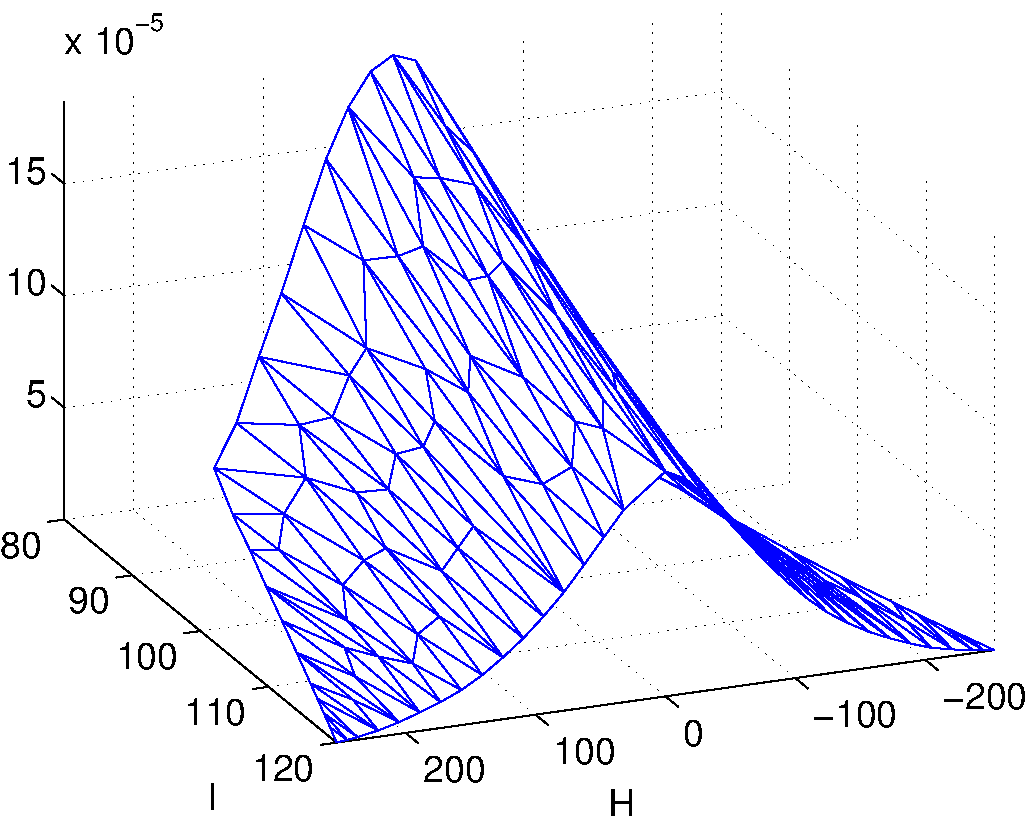
\includegraphics[width=\textwidth]{figures/fpe_solution_sigma_1_area_100}
\caption{Steady-state solution to the FPE obtained by the finite-element method when the maximum element area is 100.}
\label{f:fpe_sigma_1_area_100}
\end{center}
\end{figure}

\begin{figure}
\begin{center}
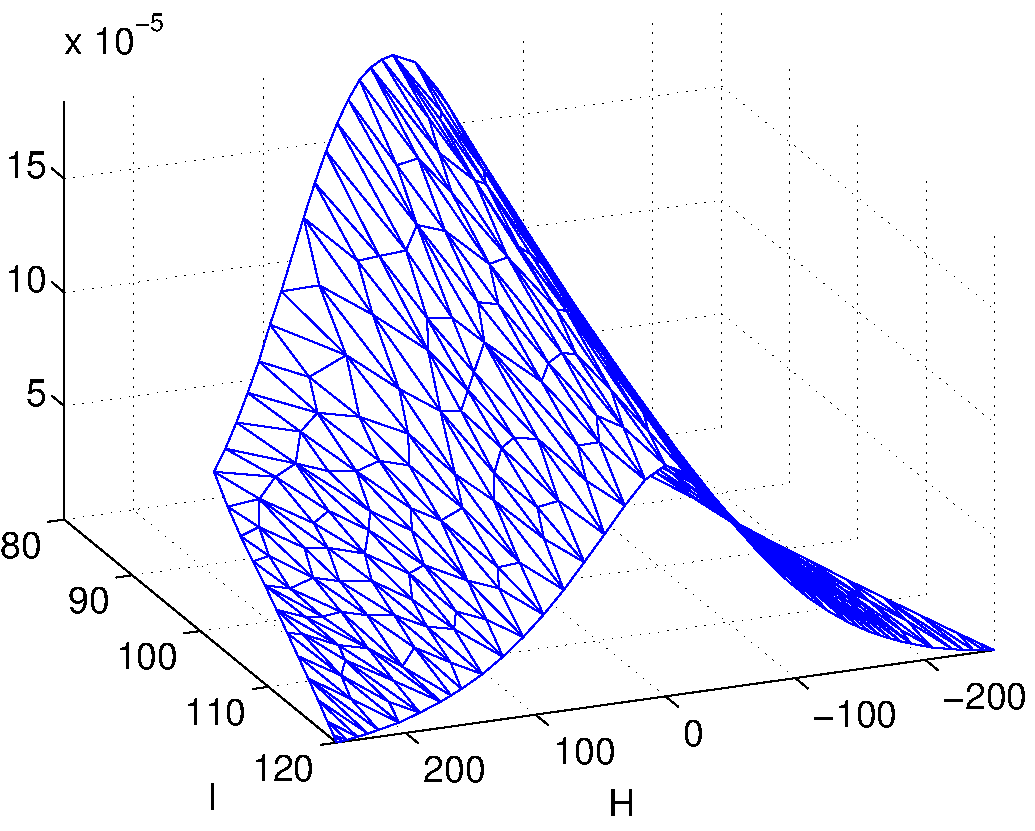
\includegraphics[width=\textwidth]{figures/fpe_solution_sigma_1_area_50}
\caption{Same solution as Figure \ref{f:fpe_sigma_1_area_100}, but with the maximum element area set to 50.}
\label{f:fpe_sigma_1_area_50}
\end{center}
\end{figure}

\begin{figure}
\begin{center}
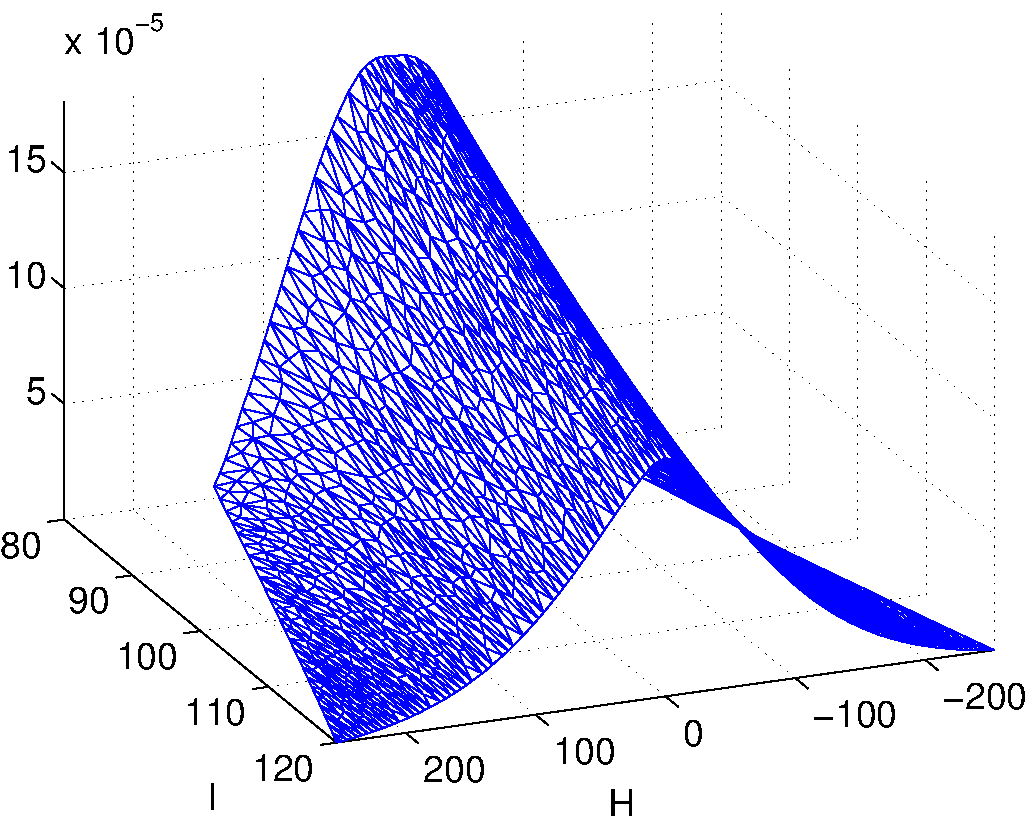
\includegraphics[width=\textwidth]{figures/fpe_solution_sigma_1_area_10}
\caption{Same solution as Figure \ref{f:fpe_sigma_1_area_100}, but with the maximum element area set to 10.}
\label{f:fpe_sigma_1_area_10}
\end{center}
\end{figure}

The next set of results is in shown in Figure \ref{f:fpe_sigma_1_i_lim}. These Figures probe the effect of varying the value of $I_\text{min}$. Recalling that the domain of the FPE has a cusp at the origin, the behavior of the solution near the origin is of interest. In Figure \ref{f:fpe_sigma_1_i_lim}, the FEM solution is plotted along the $I$-axis. Curves in that figure suggest that as the cusp is approached, the solution goes to zero.

\begin{figure}
\begin{center}
\includegraphics[width=\textwidth]{figures/autoparam_i_lim}
\caption{Steady-state solution to the FPE along $K$ = 0 for different values of $I_\text{min}$. The lines do not overlap since they use different normalization constants.}
\label{f:fpe_sigma_1_i_lim}
\end{center}
\end{figure}

The final set of solutions is shown in Figures \ref{f:fpe_sigma_.5} and \ref{f:fpe_sigma_1.5}. These figures use the same mesh as Figure \ref{f:fpe_sigma_1_area_50}, but now a physically significant parameter, the amplitude of stochastic forcing, is varied. Although there seems to be a bug in the FEM solver that causes irregularities in the solution near the gluing edge, the overall trend in the solutions seems clear. As forcing amplitude is increased, the peak of the probability distribution moves to larger values of $I$ while remaining symmetric about the $I$ axis. The latter fact is worth contemplating. Recalling the structure of the Hamiltonian, (see Figure \ref{f:autoparam Hamiltonian}) the outer edge of the domain in the left hand plane corresponds to a sink and the outer edge of the domain in the right hand plane is a valley. As such it seems reasonable to think that as forcing amplitude increases, the peak of the PDF will shift from the left hand plane to the right hand plane, but this is not observed in the Figures. In fact, simply by looking at the form of $\mathfrak b_1$ (see Equations \eqref{e:b1 valley} and \eqref{e:b1 hill} and Figure \ref{F:b1_circ}), one notices that along the $K$ axis, the drift coefficient tends to center the probability density on the $I$ axis. It is curious that $\mathfrak b_1$ does not contain any stochastic effects; whether this is a generic feature for systems in 1:2 resonance remains to be determined.

\begin{figure}
\begin{center}
\includegraphics[width=\textwidth]{figures/fpe_solution_sigma_.5.eps}
\caption{Steady-state solution to the FPE obtained by the finite-element method for $\sigma = 0.5$.}
\label{f:fpe_sigma_.5}
\end{center}
\end{figure}

\begin{figure}
\begin{center}
\includegraphics[width=\textwidth]{figures/fpe_solution_sigma_1.5.eps}
\caption{Steady-state solution to the FPE obtained by the finite-element method for $\sigma = 1.5$.}
\label{f:fpe_sigma_1.5}
\end{center}
\end{figure}
